\documentclass[a4paper, 12pt]{article}
\usepackage{deuresutils}
\usepackage{graphicx}
\graphicspath{ {images/} }

\title{Lliurament 2}
\asignatura{Càlcul en Diverses Variables}
\author{Eduardo Pérez Motato}
\niu{NIU: 1709992}
\date{25/03/2024}

\begin{document}
    \makeheader

    \setcounter{numex}{20}
    \begin{exercici}
        Decidiu si les funcions següents són diferenciables:
        \begin{itemize}
            \item[b)]
            \begin{displaymath}
                f(x,y) =
                \begin{cases}
                    \left(x^3-y^3\right)\sin{\left(\frac{1}{x^2+y^2}\right)} & \text{si } \left(x,y\right)  \neq \left(0,0\right)\\
                    0 & \text{ si} \left(x,y\right) = \left(0,0\right) 
                \end{cases}
            \end{displaymath}
        \end{itemize}
    \end{exercici}
    \begin{solucio}
        Per veure si aquesta funció és diferenciable recorrerem a la definició de diferenciabilitat,
        $f$ és diferenciable si totes les derivades parcials existeixen i $\lim\limits_{x \to x_0} \frac{f\left(x\right) - f\left(x_0\right)-\left\langle \nabla f\left(x_0\right), x-x_0\right\rangle }{\left\lVert x-x_0\right\rVert } = 0$.\\
        Primer, calculem les parcials:
        \begin{displaymath}
            \frac{\partial f}{\partial x}(x,y) = 
            \begin{cases}
                3x^2\sin{\left(\frac{1}{x^2+y^2}\right)} +  \left(x^3-y^3\right)\left(\frac{-2x}{\left(x^2+y^2\right)^2}\right)\cos{\left(\frac{1}{x^2+y^2}\right)} & \text{si } \left(x,y\right)  \neq \left(0,0\right)\\
                0 & \text{ si} \left(x,y\right) = \left(0,0\right) 
            \end{cases}
        \end{displaymath}
        \begin{displaymath}
            \frac{\partial f}{\partial y}(x,y) = 
            \begin{cases}
                3y^2\sin{\left(\frac{1}{x^2+y^2}\right)} +  \left(x^3-y^3\right)\left(\frac{-2y}{\left(x^2+y^2\right)^2}\right)\cos{\left(\frac{1}{x^2+y^2}\right)} & \text{si } \left(x,y\right)  \neq \left(0,0\right)\\
                0 & \text{ si} \left(x,y\right) = \left(0,0\right) 
            \end{cases}
        \end{displaymath}
        Veiem que existeixen, llavors ara, calculem el límit,
        \begin{displaymath}
            \begin{split}
            0 &\stackrel{?}{=} \lim\limits_{\left(x,y\right) \to \left(0,0\right)}\frac{f\left(x,y\right)-\overbrace{f\left(0,0\right)}^{ = 0}-\langle\overbrace{\nabla f\left(0, 0\right)}^{= \left(0,0\right)}, \left(x, y\right)\rangle}{\left\lVert\left(x, y\right)\right\rVert} = \lim\limits_{\left(x,y\right) \to \left(0,0\right)} \frac{f\left(x,y\right) - \overbrace{\left\langle\left(0,0\right),\left(x,y\right)\right\rangle}^{=0}}{\sqrt{x^2+y^2}}\\
              &\stackrel{?}{=} \lim\limits_{\left(x,y\right) \to \left(0,0\right)} \frac{f\left(x,y\right)}{\sqrt{x^2+y^2}} = \lim\limits_{\left(x,y\right) \to \left(0,0\right)} \frac{\left(x^3-y^3\right)\overbrace{\sin{\left(\frac{1}{x^2+y^2}\right)}}^{\in[-1, 1]}}{\sqrt{x^2+y^2}}\\
              &\stackrel{?}{=} \lim\limits_{\left(x,y\right) \to \left(0,0\right)} \frac{\left\lvert x^3-y^3\right\rvert \overbrace{\left\lvert \sin{\left(\frac{1}{x^2+y^2}\right)}\right\rvert}^{\leq 1}}{\sqrt{x^2+y^2}} \geq \lim\limits_{\left(x,y\right) \to \left(0,0\right)} \frac{\left\lvert x^3-y^3\right\rvert}{\sqrt{x^2+y^2}}\\
              &\stackrel{?}{\geq} \lim\limits_{\left(x,y\right) \to \left(0,0\right)} \frac{\left\lvert x^3-y^3\right\rvert}{\sqrt{x^2+y^2}}=\lim\limits_{\left(x,y\right) \to \left(0,0\right)} \left\lvert\frac{x^3}{\sqrt{x^2+y^2}}-\frac{y^3}{\sqrt{x^2+y^2}}\right\rvert\\
              &\stackrel{?}{\geq}\left\lvert\lim\limits_{\left(x,y\right) \to \left(0,0\right)}\frac{x^3}{\sqrt{x^2+y^2}}-\lim\limits_{\left(x,y\right) \to \left(0,0\right)}\frac{y^3}{\sqrt{x^2+y^2}}\right\rvert = \left\lvert 0 - 0\right\rvert\\
              & = 0
            \end{split}
        \end{displaymath}
        Llavors, veiem que és diferenciable.
    \end{solucio}

    \setcounter{numex}{22}
    \begin{exercici}
        En quina direcció, des del punt $\left(0,1\right)$, creix més ràpidament la funció $f(x,y) = x^2-y^2$?
    \end{exercici}
    \begin{solucio}
       Per saber això, hem de calcular $\nabla f(0,1)$ i aquest vector resultant serà el vector cap
       a on creix més ràpidament la funció en aquest punt. Primer, calculem $\nabla f$, que serà $\nabla f(x,y) = \left(\frac{\partial f}{\partial x}, \frac{\partial f}{\partial y}\right)$.\\
       En aquest cas, $\frac{\partial f}{\partial x} = 2x$ i $\frac{\partial f}{\partial y} = -2y$,
       llavors $\nabla f = \left(2x, -2y\right)$. Avaluant-ho, dona $\nabla f(0,1) = \left(0, -2\right)$.
       Llavors $\left(0, -2\right)$ és la direcció on creix més la funció $f$ al punt $\left(0, 1\right)$.
    \end{solucio}

    \setcounter{numex}{25}
    \begin{exercici}
        Sigui $f$ una funció diferenciable de $\mathbb{R}^3$ a $\mathbb{R}$. Calculeu les derivades
        que us indiquen deixant el que calgui en funció de $f$.
        \begin{itemize}
            \item[d)] Si $g(x,y,z) = f(yz, xz, xy)$, calculeu el gradient de $g$.
        \end{itemize}
    \end{exercici}
    \begin{solucio}
        Per calcular $\nabla g$, haurem de fer el ja abans dit a l'exercici anterior, però amb la
        regla de la cadena, així que farem les parcials respectives:
        \begin{displaymath}
            \frac{\partial g}{\partial x} = \frac{\partial f}{\partial (yz)} \frac{\partial (yz)}{\partial x} + \frac{\partial f}{\partial (xz)} \frac{\partial (xz)}{\partial x} + \frac{\partial f}{\partial (xy)} \frac{\partial (xy)}{\partial x}
        \end{displaymath}
        \begin{displaymath}
            \frac{\partial g}{\partial y} = \frac{\partial f}{\partial (yz)} \frac{\partial (yz)}{\partial y} + \frac{\partial f}{\partial (xz)} \frac{\partial (xz)}{\partial y} + \frac{\partial f}{\partial (xy)} \frac{\partial (xy)}{\partial y}
        \end{displaymath}
        \begin{displaymath}
            \frac{\partial g}{\partial z} = \frac{\partial f}{\partial (yz)} \frac{\partial (yz)}{\partial z} + \frac{\partial f}{\partial (xz)} \frac{\partial (xz)}{\partial z} + \frac{\partial f}{\partial (xy)} \frac{\partial (xy)}{\partial z}
        \end{displaymath}
        I ara, si simplifiquem i fem les parcials corresponents tenim:
        \begin{displaymath}
            \frac{\partial g}{\partial x} = \frac{\partial f}{\partial (xz)} z + \frac{\partial f}{\partial (xy)} y
        \end{displaymath}
        \begin{displaymath}
            \frac{\partial g}{\partial y} = \frac{\partial f}{\partial (yz)} y + \frac{\partial f}{\partial (xy)} z
        \end{displaymath}
        \begin{displaymath}
            \frac{\partial g}{\partial z} = \frac{\partial f}{\partial (yz)} y + \frac{\partial f}{\partial (xz)} x
        \end{displaymath}
        Llavors, recordant que $\nabla g = \left(\frac{\partial g}{\partial x}, \frac{\partial g}{\partial y}, \frac{\partial g}{\partial z}\right)$, aleshores:
        \begin{displaymath}
            \nabla g = \left(\frac{\partial f}{\partial (xz)} z + \frac{\partial f}{\partial (xy)} y, \frac{\partial f}{\partial (yz)} y + \frac{\partial f}{\partial (xy)} z, \frac{\partial f}{\partial (yz)} y + \frac{\partial f}{\partial (xz)} x, \right) 
        \end{displaymath}
    \end{solucio}

    \setcounter{numex}{27}
    \begin{exercici}
        Siguin $f, g : \mathbb{R}^2 \to \mathbb{R}^2$ dues funcions diferenciables. La funció $g$ ve
        donada per $g(x, y) = (x^2 - y^2, 2xy)$. Si sabem que $f(1, 3) = (2, 0)$ i que
        \begin{displaymath}
            D(g \circ f)(1,3) =
            \begin{pmatrix}
                2 & -1\\
                -3 & 4    
            \end{pmatrix},
        \end{displaymath}
        Determineu $Df(1,3)$.
    \end{exercici}
    \begin{solucio}
        Sabem que $D\left(g \circ f\right)(x) = Dg(f(x)) Df(x)$. Suposant que $Dg(f(x))$
        és invertible, podem trobar $Dg(f(x))^{-1} D\left(g \circ f\right)(x) = Df(x)$, i això és el
        que volem calcular. Llavors, calculem $Dg(f(1,3))$:
        \begin{displaymath}
            Dg =
            \begin{pmatrix}
                \frac{\partial \left(x^2-y^2\right) }{\partial x} && \frac{\partial \left(x^2-y^2\right) }{\partial y}\\
                \frac{\partial \left(2xy\right) }{\partial x} && \frac{\partial \left(2xy\right) }{\partial y}
            \end{pmatrix}
            = 
            \begin{pmatrix}
                2x && -2y\\
                2y && 2x
            \end{pmatrix}
        \end{displaymath}
        Llavors, $Dg(f(1,3)) = Dg(2,0) =
        \begin{psmallmatrix}
            4 & 0\\
            0 & 4
        \end{psmallmatrix}$.
        Aquesta matriu és, evidentment, invertible amb inversa $\begin{psmallmatrix}
            4 & 0\\
            0 & 4
        \end{psmallmatrix} = \begin{psmallmatrix}
            \frac{1}{4} & 0\\
            0 & \frac{1}{4}
        \end{psmallmatrix}$. Llavors, podem fer servir l'abans esmentat:
        \begin{displaymath}
            Df(1,3)
            =
            \begin{pmatrix}
                \frac{1}{4} & 0\\
                0 & \frac{1}{4}
            \end{pmatrix}
            \begin{pmatrix}
                2 & -1\\
                -3 & 4
            \end{pmatrix}
            = 
            \begin{pmatrix}
                \frac{1}{2} & \frac{-1}{4}\\
                \frac{-3}{4} & 1
            \end{pmatrix}
        \end{displaymath}
    \end{solucio}

    \setcounter{numex}{29}
    \begin{exercici}
        Sigui $f: \mathbb{R}^n \to \mathbb{R}$ una funció. Diem que $f$ és homogènia de grau $m$ si
        $f(tx) = t^m f(x) \forall t \in \mathbb{R}, x \in \mathbb{R}^n$.\\
        Proveu que si $f$ és diferenciable i homogènia de grau $m$, aleshores
        \begin{displaymath}
            mf(x) = \sum\limits_{j=1}^{n} x_j \frac{\partial f}{\partial x_j}(x)\hbox{ }\forall x \in \mathbb{R}^n
        \end{displaymath}
        (Indicació: Considereu la funció $g(t) = f(tx)$ i calculeu $g'(1)$.)
    \end{exercici}
    \begin{solucio}
        Seguint la indicació, calculem la derivada de $g(t)$ on $g(t) := f(tx)$:
        \begin{displaymath}
            g'(t) = f'(tx)t
        \end{displaymath}
        i com $f'(x) = Df(x)$, tenim 
        \begin{displaymath}
            g'(t) = x \cdot Df(tx)
        \end{displaymath}
        però si tenim en compte que $f$ és homogènia, podem fer el següent:
        \begin{displaymath}
            g(t) = t^m f(x)
        \end{displaymath}
        i llavors, fer un altre càlcul:
        \begin{displaymath}
            g'(t) = mt^{m-1}f(x)
        \end{displaymath}
        Ambdues $g'(t)$ les avaluem a $t = 1$, llavors ens dona el següent
        \begin{displaymath}
            \begin{split}
                g'(1) &= x \cdot Df(x)\\
                g'(1) &= m f(x)
            \end{split}
        \end{displaymath}
        Això, clarament, ha de donar el mateix, per això els igualem:
        \begin{equation}
            m f(x) = x\cdot Df(x)
            \label{eq:1}
        \end{equation}
        Això s'assembla molt al que havíem de demostrar, i amb una mica d'ull ens adonem que es
        exactament equivalent a causa de com es multipliquen els, en aquest cas de $f: \mathbb{R}^n\to\mathbb{R}$,
        vectors. Com $Df(x) = \left(\frac{\partial f}{\partial x_1}(x), \frac{\partial f}{\partial x_2}(x), \dots, \frac{\partial f}{\partial x_n}(x)\right)$,
        la multiplicació de vectors és $\sum\limits_{j=1}^{n} x_j \frac{\partial f}{\partial x_j}(x)$.
        Si això ho posem a \eqref{eq:1}, ens queda el següent:
        \begin{displaymath}
            mf(x) = \sum\limits_{j=1}^{n} x_j \frac{\partial f}{\partial x_j}(x)
        \end{displaymath}
        I això era el que volíem demostrar.
    \end{solucio}
    
    \setcounter{numex}{32}
    \begin{exercici}
        Proveu que no hi ha cap punt de la superfície $xyz = 1$ on el vector normal sigui horitzontal.
    \end{exercici}
    \begin{solucio}
        El vector normal de la superfície $xyz = 1$ el calcularé fent $Df(x,y,z)$, on $f(x,y,z) = xyz$.
        \begin{obs}
            Com el concepte "horitzontal" em sembla ambigu, comprovaré que exactament dos vectors de $\left\{OX, OY, OZ\right\}$
            en fer el producte escalar el resultat sigui $0$.
        \end{obs}
        Com $Df = \left(\frac{\partial f}{\partial x}, \frac{\partial f}{\partial y}, \frac{\partial f}{\partial z}\right)$,
        calculem les derivades parcials següents:
        \begin{displaymath}
            \begin{split}
                \frac{\partial f}{\partial x} &= yz\\
                \frac{\partial f}{\partial y} &= xz\\
                \frac{\partial f}{\partial z} &= xy
            \end{split}
        \end{displaymath}
        Recordant que $xyz = 1$, posem aquesta restricció en la nostra $Df$ avaluant $\left(\frac{1}{yz}, y, z\right)$
        \begin{displaymath}
            Df\left(\frac{1}{yz}, y, z\right) = \left(yz, \frac{1}{y}, \frac{1}{z}\right)  
        \end{displaymath}
        Amb aquest vector resultant podem veure que per fer que el producte escalar sigui igual a $0$
        és imposible, degut al següent:
        \begin{itemize}
            \item $\left\langle OX, \left(yz, \frac{1}{y}, \frac{1}{z}\right)\right\rangle = 0 \iff yz = 0$,
            per això $y = 0$ o $z = 0$. Ambdues opcions són invàlides ja que provocaría problemes a
            $\frac{1}{y}$ o $\frac{1}{z}$.
            \item $\left\langle OY, \left(yz, \frac{1}{y}, \frac{1}{z}\right)\right\rangle = 0 \iff \frac{1}{y} = 0$,
            i això no passa mai.
            \item Anàlogament, $\left\langle OZ, \left(yz, \frac{1}{y}, \frac{1}{z}\right)\right\rangle = 0 \iff \frac{1}{z} = 0$,
            i això tampoc passa mai.
        \end{itemize}
    \end{solucio}

    \setcounter{numex}{35}
    \begin{exercici}
        Considerem la corba $\gamma(t) = ((t^2-t+2)\cos{(2\pi t)}, (t^2-t+2)\sin{(2\pi t)}), t \in [0, 1]$.
        \begin{enumerate}[label=\alph*)]
            \item Feu un dibuix de $\gamma(t)$.\\
            \begin{solucio}
                Primer veiem on creua els eixos. En els eixos de les $x$, $y$ ha de ser equivalent a $0$,
                és dir $(t^2-t+2)\sin{(2\pi t)} = 0$, en aquest cas o $t^2-t+2 = 0$ o $\sin{(2\pi t)} = 0$.
                $t^2-t+2 = 0 \iff t \not\in \mathbb{R}$ i $\sin{(2\pi t)} = 0 \iff t = \frac{n}{2},\; n \in \mathbb{Z}$.
                Llavors, $t \in \left\{0, \frac{1}{2}, 1\right\}$.\\
                En els eixos de les $y$, $x$ ha de ser equivalent a $0$, és dir $(t^2-t+2)\cos{(2\pi t)} = 0$,
                també en aquest cas només té solució real a $t = \frac{n}{2} - \frac{1}{4},\; n\in \mathbb{Z}$.
                Llavors, $t \in \left\{\frac{1}{4}, \frac{3}{4}\right\}$. Aquests punts són $\left\{\left(0, 2\right), \left(0, -\frac{7}{4}\right), \left(0, 2\right), \left(\frac{29}{16}, 0\right), \left(-\frac{29}{16}, 0\right)\right\}$.\\
                El gràfic resultant és aquest:
                \begin{center}
                    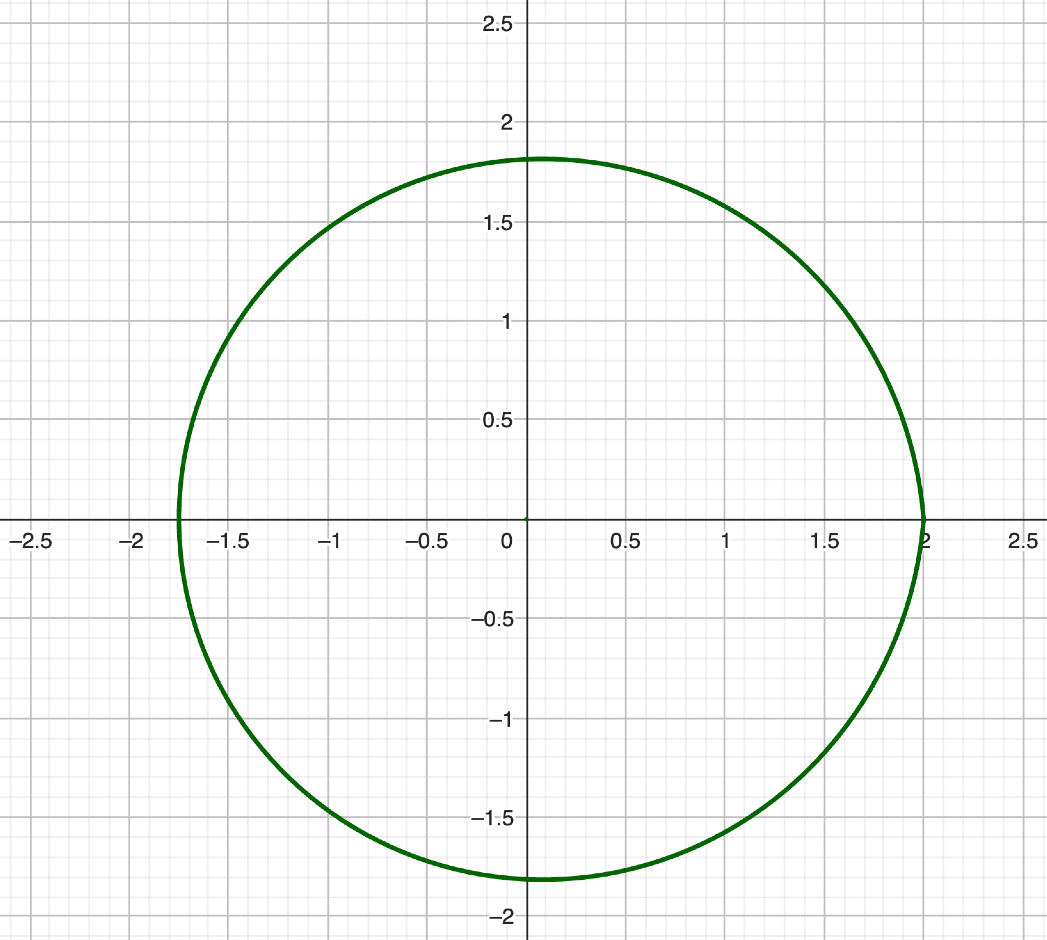
\includegraphics[width=0.5\textwidth]{Grafica.png}\\
                    Fet amb GeoGebra, ja que LaTeX no el genera bé.
                \end{center}
            \end{solucio}
            \item Determineu quin punt de $\gamma(t)$ està més lluny de l'origen.\\
            \begin{solucio}
                Per fer això, calcularem $\left\lVert\gamma(t)-\left(0,0\right)\right\rVert$, o el
                que és equivalent, $\left\lVert\gamma(t)\right\rVert$. Això és el següent:
                \begin{displaymath}
                    \begin{split}
                        \left\lVert\gamma(t)\right\rVert &= \sqrt{\left((t^2-t+2)\sin{(2\pi t)}\right)^2+\left((t^2-t+2)\cos{(2\pi t)}\right)^2}\\
                        &= \sqrt{(t^2-t+2)^2\sin^2{(2\pi t)}+(t^2-t+2)^2\cos^2{(2\pi t)}}\\
                        &= \sqrt{(t^2-t+2)^2\left(\sin^2{(2\pi t)}+\cos^2{(2\pi t)}\right)}\\
                        &= t^2-t+2
                    \end{split}
                \end{displaymath}
                Gràcies a això, sabem que $\left\lVert\gamma(t)\right\rVert$ és, òbviament, continua
                i derivable. Ara, derivem per trobar on són els extrems relatius,
                \begin{displaymath}
                    \left\lVert\gamma(t)\right\rVert' = 2t-1
                \end{displaymath}
                $\left\lVert\gamma(t)\right\rVert' = 0 \iff t = \frac{1}{2}$. Llavors, ara mirem els
                extrems de definició i els extrems relatius:
                \begin{center}
                    \begin{tabular}[h]{|c|c|}
                        \hline
                        $t$ & $\gamma(t)$\\
                        \hline
                        $0$ & $2$\\
                        $\frac{1}{2}$ & $\frac{7}{4}$\\
                        $1$ & $2$\\
                        \hline
                    \end{tabular}
                \end{center}
                Llavors, veiem com els punts més lluny de l'origen corresponen amb $t = 0$ o $t=1$\\
                Aquests punts, més ben dit, aquest punt (ja que és el mateix) és $\left(0,2\right)$. 
            \end{solucio}
            \item Determineu el vector tangent a la corba en el punt anterior.\\
            \begin{solucio}
                El vector tangent es treu mitjançant $\dot{\gamma}(t)$:
                \begin{displaymath}
                    \dot{\gamma}(t) =
                    \begin{pmatrix}
                        \left(2t-1\right)\cos{\left(2\pi t\right)}-2\pi\left(t^2-t+2\right)\sin{\left(2\pi t\right)}\\
                        \left(2t-1\right)\sin{\left(2\pi t\right)}+2\pi\left(t^2-t+2\right)\cos{\left(2\pi t\right)}
                    \end{pmatrix}
                \end{displaymath}
                Si avaluem $\dot{\gamma}(0)$, tenim
                \begin{displaymath}
                    \dot{\gamma}(0) = \left(-1, 4\pi\right)
                \end{displaymath}
                Notem que si avaluem $\dot{\gamma}(1)$, tenim
                \begin{displaymath}
                    \dot{\gamma}(1) = \left(1, 4\pi\right)
                \end{displaymath}
                Aquests vectors no són pas equivalents, per això, no existeix com tal.
            \end{solucio}
            \item Per al punt anterior, determineu l'angle que formen la posició i la velocitat.\\
            \begin{solucio}
                Per fer això, farem servir $\cos{\alpha} = \frac{\left\langle\gamma(0), \dot{\gamma}(0)\right\rangle}{\left\lVert \gamma(0)\right\rVert \left\lVert \dot{\gamma}(0)\right\rVert }$
                \begin{displaymath}
                    \cos{\alpha} = \frac{\left\langle\left(0,2\right) , \left(1, 4\pi\right)\right\rangle}{\left\lVert \left(0,2\right) \right\rVert \left\lVert \left(1, 4\pi\right) \right\rVert} = \frac{4\pi}{2\sqrt{1+16\pi^2}}
                \end{displaymath}
                Si invertim el $\cos$, tenim $\alpha$:
                \begin{displaymath}
                    \alpha = \arccos{\left(\frac{4\pi}{2\sqrt{1+16\pi^2}}\right)} \approx 1.0490160175847 \text{ rad} = 60.1041904492239^o
                \end{displaymath}
            \end{solucio}
        \end{enumerate}
    \end{exercici}
\end{document}